\documentclass[article,A4,12pt]{llncs}
\usepackage[T1]{fontenc}
\usepackage{amsmath}
\usepackage{amssymb}
\usepackage{amsfonts}
\usepackage{mathrsfs, bm}

\usepackage{graphicx}
\usepackage{tabularx}
\usepackage{subfig}
\usepackage{epsf,times}
\usepackage{color}
\usepackage{wrapfig}
\usepackage{cases}
\usepackage{multicol}

\usepackage[T1]{fontenc}
%\newcommand{\tmname}[1]{\textsc{#1}}
%\newcommand{\tmop}[1]{\ensuremath{\operatorname{#1}}}
%\newcommand{\tmsamp}[1]{\textsf{#1}}
%\newcommand{\tmtextsc}[1]{{\scshape{#1}}}
%\newcommand{\tmtextsl}[1]{{\slshape{#1}}}
%\newcommand{\tmtexttt}[1]{{\ttfamily{#1}}}

\leftmargin=0.0cm
\oddsidemargin=0.5cm
\evensidemargin=0.5cm
\topmargin=0cm
\textwidth=16.0cm
%\textheight=21.5cm
\textheight=20.0cm
\pagestyle{plain}
\setlength{\columnsep}{20pt}

\def\m{\mathbf{m}}
\def\H{\mathbf{H}}
\def\E{\mathbf{E}}
\newcommand{\vepsi}{{\varepsilon}}
\def\hnorm#1#2{\vert\,#1\,\vert_{#2}}
\newcommand{\R}{{\mathbb R}}
\newcommand{\Sph}{{\mathbb S}}
\def\x{\mathbf{x}}
\def\hvec{\overline{\mathbf{h}}}
\def\evec{\overline{\mathbf{e}}}

\newcommand{ \etal}{\mbox{\emph{et al. }}}

\newcommand\vect[1]{\mbf{#1}}
\newcommand{\mbf}[1]{\mbox{\boldmath$#1$}} 
\newcommand{\RC}[1]{#1 $\times$ #1 $\times$ #1}
\def\um{$\mu$m}
\def\C{$^{\circ}\mathrm{C}$}

\newcommand{\Rmnum}[1]{\expandafter\@slowromancap\romannumeral #1@}

% DEFINITION OF CUSTOM FONT SIZE
\newcommand{\customfontA}{\fontsize{50}{55}\selectfont}
\newcommand{\customfontB}{\fontsize{14.4}{20}\selectfont}
\newcommand{\customfontC}{\fontsize{30}{35}\selectfont}

\DeclareMathAlphabet{\mathpzc}{OT1}{pzc}{m}{it}

\def\clovek#1{\noindent\bgroup\vbox{\noindent#1}\egroup\vskip1em}

% TO INPUT BACKGROUND IMAGE
\usepackage{eso-pic}
\newcommand\BackgroundPic{
\put(0,0){
\parbox[b][\paperheight]{\paperwidth}{
\vfill
\centering
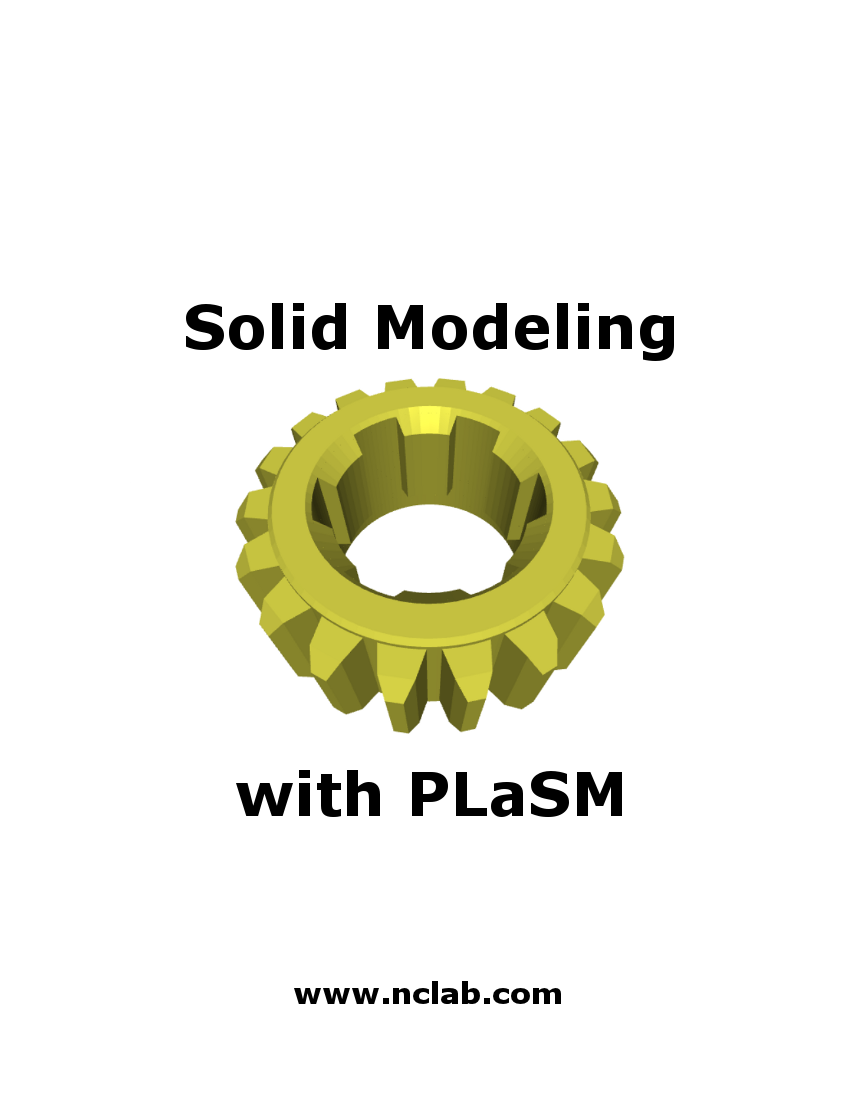
\includegraphics[width=\paperwidth,height=\paperheight]{img/plasm-frontpage.png}
%\includegraphics[width=\paperwidth,height=\paperheight]{img/background.jpg}
\vfill
}}}

\begin{document}

% INPUTTING BACKGROUND IMAGE
\AddToShipoutPicture{\BackgroundPic}
\vbox{}
\pagestyle{empty}
\newpage
\textwidth=15.5cm
\ClearShipoutPicture
\newpage

%%%%%%%%%%%%%%%%%%%%%%%%%%%%%%%%%%%%%%%%%%%%%%%%%%%%%%%%%%%%%%%%%%%%%%%%%

\section*{}
\small
\subsection*{About NCLab}
Networked Computing Laboratory (NCLab) is a popular Internet-based framework for 
programming, mathematics, computer modeling, 
and scientific computing. It serves students, instructors, researchers, and the general 
public. NCLab can be used free of charge for personal non-commercial purposes such as 
private hobby or self-education, as well as for individual non-funded academic research.
All other use is subject to {\bf purchasing a license} for a symbolic fee. The fees are as low as 
\$1 per user per month for educational use, and they are used to support the development 
and operational expenses. NCLab is a product of FEMhub Inc. The name "NCLab" is 
registered with the U.S. Patent and Trademark Office (USPTO) under Trademark No. 85420518.

\subsection*{Terms of Use and Pricing}
More details on purchasing a license and using NCLab are provided in the online documents 
{\bf Pricing} and {\bf Terms of Use} that are accessible from NCLab's home page 
{\tt http://nclab.com}.

\subsection*{Contact Information}
General inquiries: {\tt info@femhub.com}\\
Sales: {\tt sales@femhub.com}\\
NCLab support: {\tt support@nclab.com}\\
Agros \& Hermes support: {\tt support@femhub.com}\\
Web page: {\tt http://femhub.com}\\
{Physical address}\\
FEMhub Inc.\\
5490 Twin Creeks Dr.\\
Reno, NV 89523

\subsection*{About This Publication}
This publication can be copied and distributed without any restrictions
as long as reference to NCLab and FEMhub Inc. is preserved.

\subsection*{Acknowledgement}
This publication features PLaSM, an open source Programming Language for 
Solid Modeling, developed by Alberto Paoluzzi, Giorgio Scorzelli, and their 
students and collaborators at the University of Rome in Italy. Alberto's 
and Giorgio's help and support are gratefully acknowledged. 

\normalsize

\newpage
%{\ }
\setcounter{tocdepth}{2}
\tableofcontents
%\pagestyle{plain}

\newpage

\pagestyle{plain}
\setcounter{page}{1}

%%%%%%%%%%%%%%%%%%%%%%%%%%%%%%%%%%%%%%%%%%%%%%%%%%%%%%%%%%%%%%%%%%%%%%%%%

\section{What is PLaSM?}

PLaSM ({\em Programming Language for Solid Modeling}) is a design language
that enables geometrical modeling of 3D objects via simple commands.
The language was developed by the CAD Group at the Universities of Roma 
"La Sapienza" and "Roma Tre" in Italy. It is based on FL, an advanced 
language for functional programming developed by the Functional 
Programming Group at the IBM Research Center.\\

\noindent
PLaSM makes it possible to define a wide range of simple 3D objects, transform 
them, create intersections and unions via simple logical operations, and much 
more. This tutorial will guide you in small steps and using many examples
through PLaSM's usage. Soon, you will be able to create advanced 
3D geometries such as the one shown in Fig. \ref{fig:pisa}.

\begin{figure}[!ht]
\begin{center}
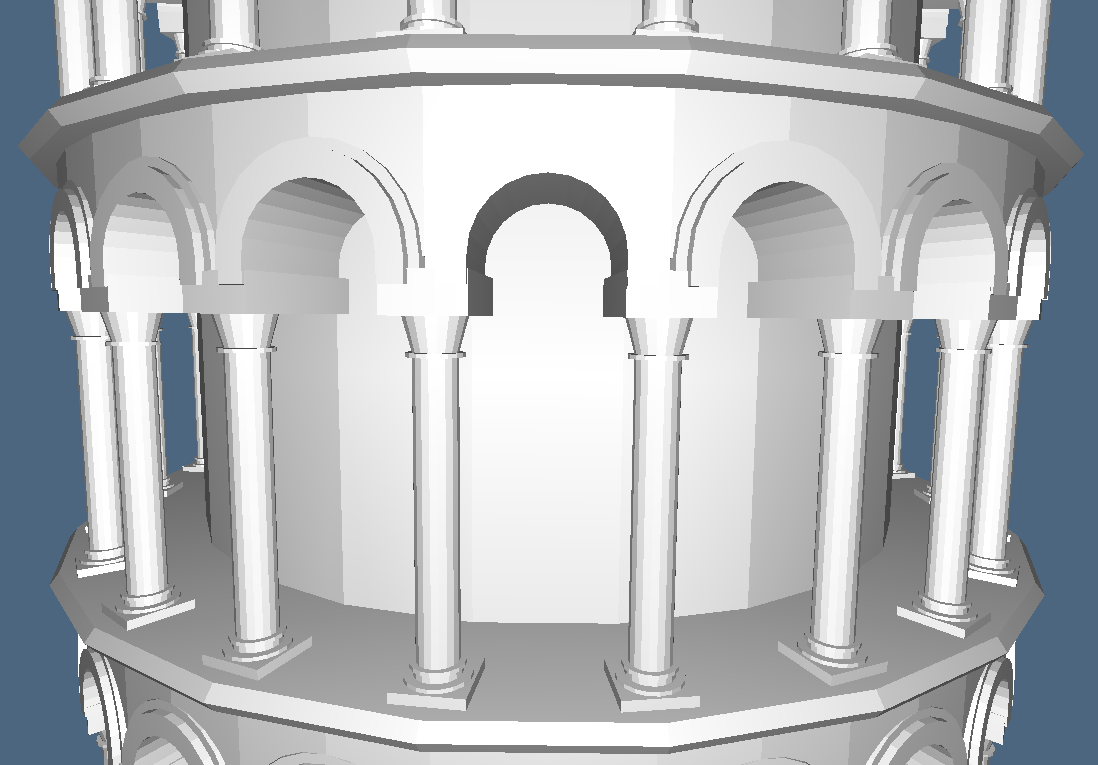
\includegraphics[width=0.8\textwidth]{img/pisa.png}
\end{center}
\vspace{-2mm}
\caption{Snapshot of a PLaSM model of the famous Pisa Tower.}
\label{fig:pisa}
\end{figure}

\section{Getting Started}

In order to make the most of this tutorial, we invite the 
reader to create an account in NCLab and log in. More instructions 
on how to do this are given at the beginning of the introductory 
tutorial "Meet Your New Graphing Calculator" that is available in 
PDF via a link on NCLab home page {\tt http://nclab.com}. \\

\noindent
{\bf NOTE}: Your web browser needs to support WebGL, otherwise you will not be able to 
work with PLaSM properly. For this reason, a WebGL tester is provided 
on NCLab's front page.\\

\noindent
After logging in, you will see a PC-like desktop with several icons on it,
as shown in Fig. \ref{fig:desktop}. 

\begin{figure}[!ht]
\begin{center}
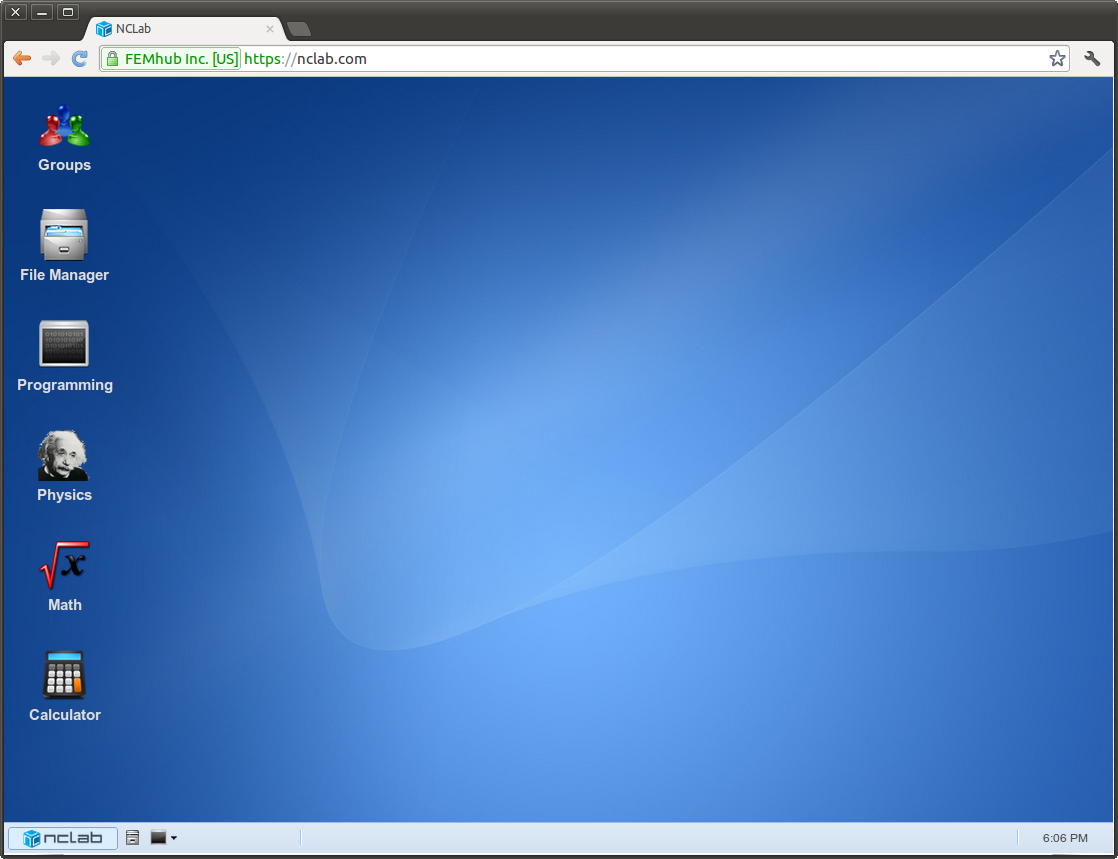
\includegraphics[width=\textwidth]{img/desktop.png}
\end{center}
%\vspace{-2mm}
\caption{NCLab desktop after login.}
\label{fig:desktop}
\end{figure}

\subsection{Launching a new Python project}

Click on the File Manager icon. This will launch the File Manager.
In the Project menu choose New $\rightarrow$ Python. This will launch an 
empty Python project, as shown in Fig. \ref{fig:python}.

\newpage

\begin{figure}[!ht]
\begin{center}
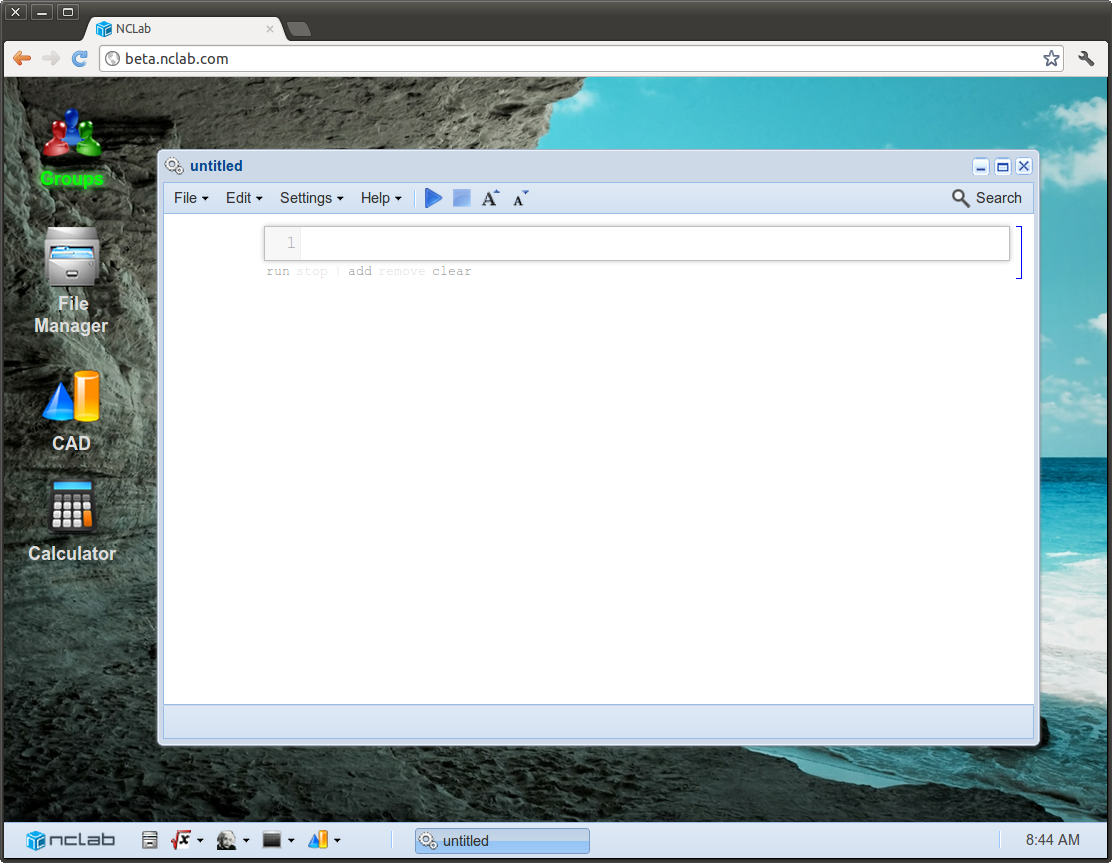
\includegraphics[width=\textwidth]{img/python.png}
\end{center}
%\vspace{-2mm}
\caption{Launching a new Python project.}
\label{fig:python}
\end{figure}
\noindent

\subsection{Creating a unit cube}

In the input cell, enter the code:

\begin{verbatim}
from pyplasm import *
cube = CUBOID([1, 1, 1])
lab.view(cube, [0.4, 0.9, 0.6])
\end{verbatim}
Then click on the link "run" under the input cell. This will send a request 
to the cloud. The answer should come back instantly, and a new WebGL widget 
with a unit cube in it should appear, as shown in Fig. \ref{fig:cube}. 
Congratulations, you just created your first PLaSM model!

\newpage

\begin{figure}[!ht]
\begin{center}
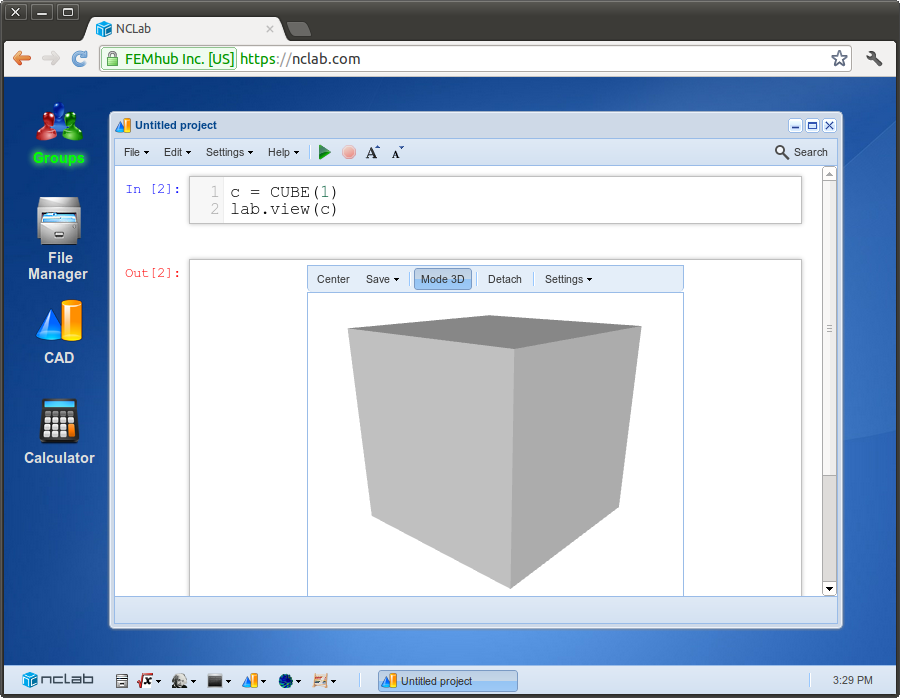
\includegraphics[width=\textwidth]{img/cube.png}
\end{center}
%\vspace{-2mm}
\caption{WebGL widget containing a unit cube.}
\label{fig:cube}
\end{figure}

\subsection{Mouse controls}

Now click into the window and move the mouse while holding the left
button pressed. The cube should freely rotate in 3D. Holding the middle
button (or the mouse wheel) pressed and moving the mouse will move the 
object to any direction. Zooming can be done with the mouse wheel or
with the right-hand mouse button.

\section{Creating Simple Objects}

Before we move on, let us briefly explain the above code.
The first line, 

\begin{verbatim}
from pyplasm import *
\end{verbatim}
imports the PLaSM library into NCLab. This is similar to how we imported
the Sympy, Numpy and Scipy libraries in the introductory course "Meet Your 
New Graphing Calculator". The second line,

\begin{verbatim}
cube = CUBOID([1, 1, 1])
\end{verbatim}
defines a 3D unit cube. The CUBOID command will be explained in more detail below.
The last line,

\begin{verbatim}
lab.view(cube, [0.4, 0.9, 0.6])
\end{verbatim}
tells NCLab to display the cube in a WebGL widget. 

\subsection{Using colors}

The triplet {\tt [0.4, 0.9, 0.6]} in the {\tt lab.view()} command
represents the RGB components defining a color. The numbers need to be between 
0.0 and 1.0. You can experiment with colors, keeping a few simple rules in mind:

\begin{itemize}
\item With just the first value being non-zero, such as in {\tt [0.5, 0, 0]},
      you get {\bf red} color. The closer the value is to 1.0, the lighter the color
      will be.
\item With just the second value being non-zero, such as in {\tt [0, 0.5, 0]},
      you obtain {\bf green} color. The closer the  value is to 1.0, the lighter the color
      will be.
\item With just the third value being non-zero, such as in {\tt [0, 0, 0.5]},
      you will have {\bf blue} color. The closer the  value is to 1.0, the lighter the color
      will be.
\item Using three identical values will result into a shade of grey. {\tt [0, 0, 0]}
      means black, {\tt [1.0, 1.0, 1.0]} means white.
\item Varying all three numbers, you can get any color that you want. It is not 
      easy to translate a color, such as "purple", "cyan" or "orange" into the RGB
      values. But there are many web pages that will do it for you, such as for
      example http://kb.iu.edu/data/aetf.html. {\bf Note}: Usually,
      the RGB values on these web pages are given as integers between 0 and 255. To use them in NCLab,
      just divide all three of them by 255.
\end{itemize}

 
\subsection{Brick, cube, rectangle, and square -- command CUBOID}

Why is the command called 
CUBOID and not CUBE? The answer is -- because the command covers more 
than cubes. With three parameters {\tt [a, b, c]} it will render 
a 3D brick with edge lengths {\tt a}, {\tt b} and {\tt c}. Let us change the 
above code to  

\begin{verbatim}
from pyplasm import *
cube = CUBOID([3, 2, 1])
lab.view(cube, [0.4, 0.9, 0.6])
\end{verbatim}
and press the "run" link under the input cell again. The result is 
displayed in Fig. \ref{fig:cuboid-1}.

\newpage

\begin{figure}[!ht]
\begin{center}
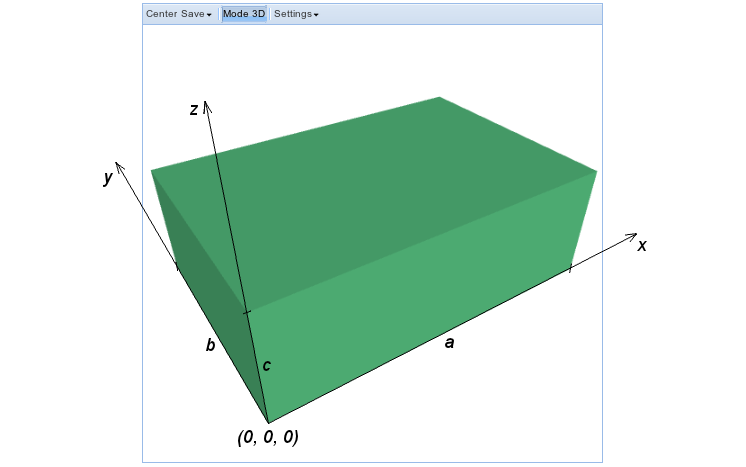
\includegraphics[width=0.8\textwidth]{img/cuboid-1.png}
\end{center}
\vspace{-2mm}
\caption{CUBOID([3, 2, 1]) generates a brick with edge lenghts 3, 2 and 1.}
\label{fig:cuboid-1}
\end{figure}
\noindent
With two parameters {\tt [a, b]} the CUBOID command will render a 2D rectangle 
(2D brick if you like) with edge lengths {\tt a} and {\tt b}, as shown in 
Fig. \ref{fig:cuboid-2}

\begin{figure}[!ht]
\begin{center}
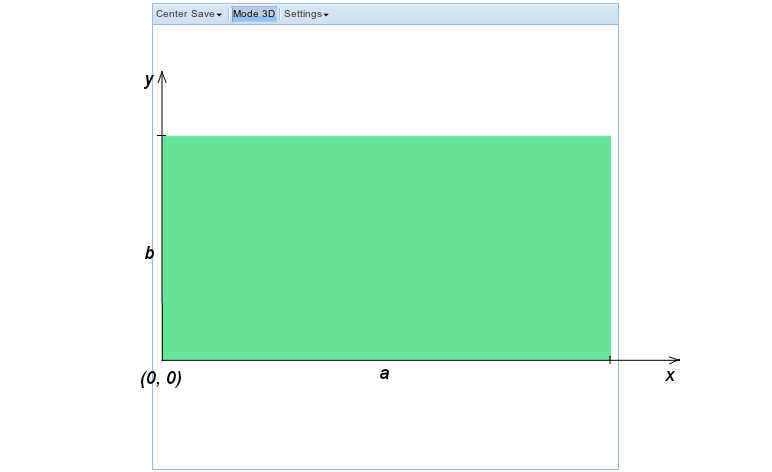
\includegraphics[width=0.82\textwidth]{img/cuboid-2.png}
\end{center}
\vspace{-2mm}
\caption{CUBOID([2, 1]) generates a rectangle with edge lenghts 2 and 1.}
\label{fig:cuboid-2}
\vspace{-1cm}
\end{figure}
\newpage


\subsection{Unit tetrahedron and triangle -- command SIMPLEX}

A unit tetrahedron (unit 3D simplex) can be created using the code
\begin{verbatim}
from pyplasm import *
tet = SIMPLEX(3)
lab.view(tet, [0.4, 0.9, 0.6])
\end{verbatim}
The result is shown in Fig. \ref{fig:simplex-1}.

\begin{figure}[!ht]
\begin{center}
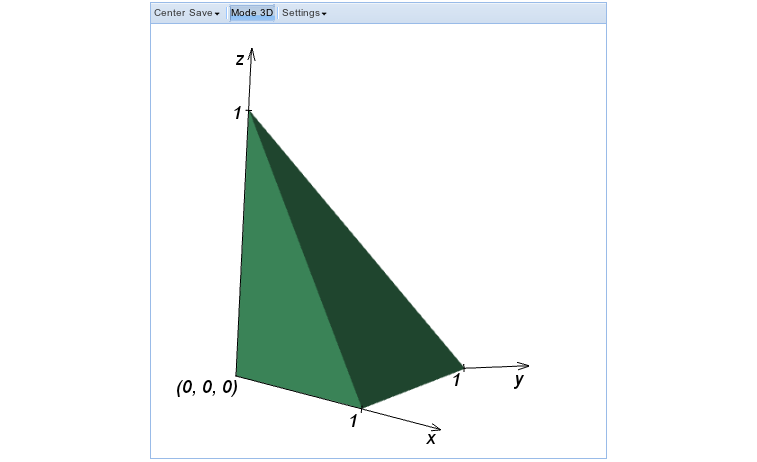
\includegraphics[width=0.82\textwidth]{img/simplex-1.png}
\end{center}
\vspace{-2mm}
\caption{SIMPLEX(3) generates a unit 3D simplex (unit tetrahedron).}
\label{fig:simplex-1}
\end{figure}
\noindent
Note -- in the next paragraph we will show how to create a general 
tetrahedron using the 
A unit triangle (unit 2D simplex) can be created using the code
\begin{verbatim}
from pyplasm import *
tria = SIMPLEX(2)
lab.view(tria, [0.4, 0.9, 0.6])
\end{verbatim}
The result is shown in Fig. \ref{fig:simplex-2}.
\newpage

\begin{figure}[!ht]
\begin{center}
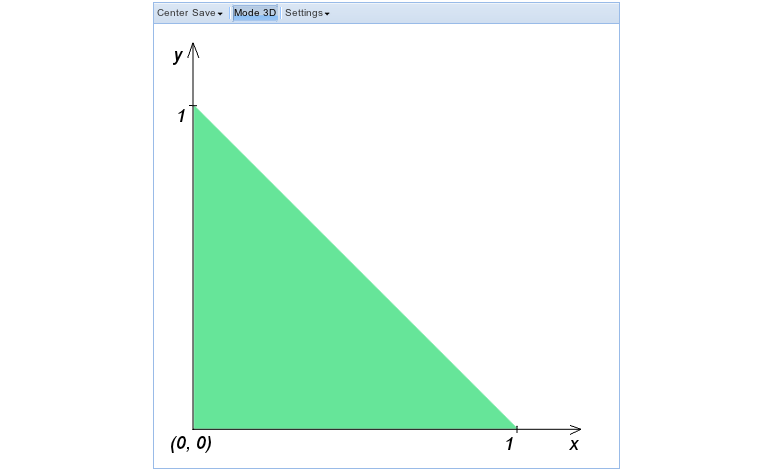
\includegraphics[width=0.82\textwidth]{img/simplex-2.png}
\end{center}
\vspace{-2mm}
\caption{SIMPLEX(2) generates a unit 2D simplex (triangle).}
\label{fig:simplex-2}
\vspace{-1cm}
\end{figure}

\subsection{General tetrahedron and triangle}

The command CONVEXHULL is a powerful tool to define convex 3D and 2D objects using 
their corner points. In particular it can be used to create general tetrahedra and 
triangles. The command takes a list of points as an argument. For example, the code

\begin{verbatim}
from pyplasm import *
points = [[-1, 0, 0], [1, 0, 0], [0, 4, 1], [0, 1, 5]]
tetra = CONVEXHULL(points)
lab.view(tetra, [0.4, 0.9, 0.6])
\end{verbatim}
creates a tetrahedron with vertices $[-1, 0, 0]$, $[1, 0, 0]$, $[0, 4, 1]$ and $[0, 1, 5]$.
The code

\begin{verbatim}
from pyplasm import *
points = [[1, 1], [4, 2], [2, 4]]
tria = CONVEXHULL(points)
lab.view(tria, [0.4, 0.9, 0.6])
\end{verbatim}
generates a triangle with the vertices $[1, 1]$, $[4, 2]$ and $[2, 4]$. In this way 
the reader can define any convex polytop in 3D or polygon in 2D -- just using more 
points!

\subsection{Convex hull -- command CONVEXHULL}


But let us 
demonstrate the true power of PLaSM by writing a simple program that generates 
a polygon with $N$ equally-long edges that is inscribed into a circle of radius $R$:

\begin{verbatim}
from pyplasm import *
from numpy import sin, cos, pi
N = 15
R = 5
points = []
for i in range(N):
    angle = i * 2. * pi / N
    points.append([R * cos(angle), R * sin(angle)])
polygon = CONVEXHULL(points)
lab.view(polygon, [0.4, 0.9, 0.6])
\end{verbatim}
The result is shown in Fig. \ref{fig:convexhull-1}.

\begin{figure}[!ht]
\begin{center}
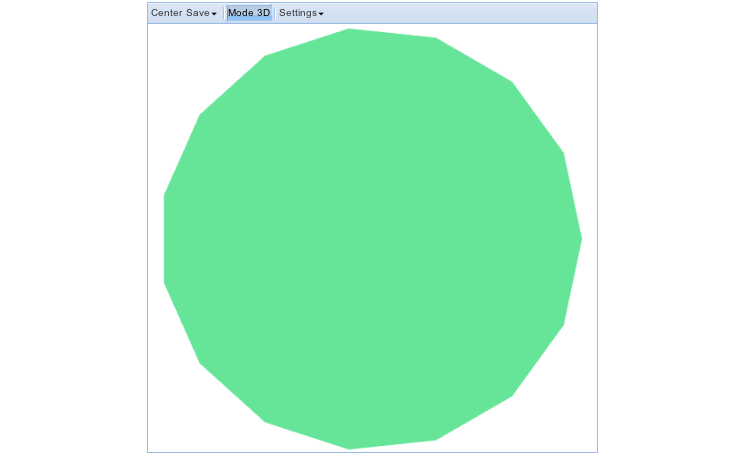
\includegraphics[width=0.82\textwidth]{img/convexhull-1.png}
\end{center}
\vspace{-2mm}
\caption{Polygon with 15 equally long edges inscribed into a circle.}
\label{fig:convexhull-1}
%\vspace{-1cm}
\end{figure}
\noindent
Feel free to experiment with various values of $N$ and $R$.
For this example, you need to know elementary commands of the Python programming 
language. If you have never programmed in Python, do not worry and skip to the next 
example. Eventually, read the tutorial on Python Programming that is also provided.

\subsection{Cone via convex hull}

The CONVEXHULL command has amazing power. Let us tweak the code
from the previous paragraph a bit to construct a cone of radius
$R$ and height $H$. All we need to do is to add a zero third coordinate 
to the points generated in the previous program, and add one more 
point -- the tip of the cone:

\begin{verbatim}
from pyplasm import *
from numpy import sin, cos, pi
R = 5
H = 10
points = []
subdiv = 128
for i in range(N):
    angle = i * 2. * pi / subdiv
    points.append([R * cos(angle), R * sin(angle), 0])
points.append([0, 0, H])
cone = CONVEXHULL(points)
lab.view(cone, [0.4, 0.9, 0.6])
\end{verbatim}
The result is shown in Fig. \ref{fig:convexhull-2}.

\begin{figure}[!ht]
\begin{center}
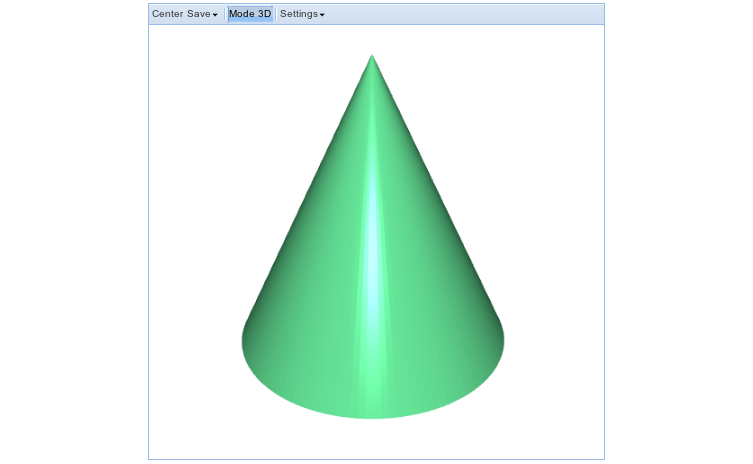
\includegraphics[width=0.82\textwidth]{img/convexhull-2.png}
\end{center}
\vspace{-2mm}
\caption{Cone of radius $R$ and height $H$.}
\label{fig:convexhull-2}
%\vspace{-1cm}
\end{figure}
\noindent
\subsection{Cylinder -- command CYLINDER}



\subsection{Tube -- command TUBE}


\subsection{Sphere -- command SPHERE}



\subsection{Torus -- command TORUS}



\subsection{Star -- command STAR}



\subsection{Extrusion of 2D objects into 3D -- commands QUOTE and POWER}





\section{Transformations}





\section{Intersections, Unions, and Such}




\section{Examples}


\end{document}
